\documentclass[10pt]{article}

% ------------------------------------------------------------------
%  "Tmux Is All You Need" -- NeurIPS-2017-style single-column layout,
%  mirroring the structure of Vaswani et al., "Attention Is All You Need".
% ------------------------------------------------------------------

\usepackage[letterpaper,margin=1in,top=1in,bottom=1in]{geometry}
\usepackage{mathptmx}            % Times-like text + math (NeurIPS look)
\usepackage[T1]{fontenc}
\usepackage[utf8]{inputenc}
\usepackage{amsmath,amssymb}
\usepackage{booktabs}
\usepackage{array}
\usepackage{microtype}
\usepackage{titlesec}
\usepackage{listings}
\usepackage{xcolor}
\usepackage{graphicx}
\usepackage{tikz}
\usetikzlibrary{positioning,fit,arrows.meta,calc}
\usepackage[hidelinks]{hyperref}

% --- Section styling reminiscent of the NeurIPS template -----------
\titleformat{\section}{\normalfont\large\bfseries}{\thesection}{0.6em}{}
\titleformat{\subsection}{\normalfont\normalsize\bfseries}{\thesubsection}{0.6em}{}
\titleformat{\subsubsection}{\normalfont\normalsize\itshape}{\thesubsubsection}{0.6em}{}
\titlespacing*{\section}{0pt}{1.6ex plus 1ex minus .2ex}{1.0ex plus .2ex}

% --- Listing style for shell / tmux commands -----------------------
\definecolor{codebg}{gray}{0.96}
\definecolor{codecomment}{rgb}{0.35,0.45,0.35}
\lstdefinestyle{sh}{
  basicstyle=\ttfamily\footnotesize,
  backgroundcolor=\color{codebg},
  commentstyle=\color{codecomment}\itshape,
  breaklines=true,
  breakatwhitespace=false,
  columns=fullflexible,
  keepspaces=true,
  frame=none,
  xleftmargin=0.6em,
  aboveskip=1ex,belowskip=1ex,
  morecomment=[l]{\#},
  literate={~}{{\raisebox{-0.5ex}{\textasciitilde}}}1
}
\lstset{style=sh}

\newcommand{\code}[1]{\texttt{\small #1}}

\setlength{\parskip}{0.4ex}
\setlength{\parindent}{0pt}

% ------------------------------------------------------------------
\begin{document}

\begin{center}
  {\LARGE\bf Tmux Is All You Need}\\[0.4em]
  {\large A Terminal-Multiplexer Architecture for Recursive Coding-Agent Orchestration}\\[1.2em]
  {\large Fabio Pauli\thanks{Human-in-the-loop. Equal contribution asserted, sequentially, by every agent in the swarm.}}\\[0.2em]
  {\ttfamily apritzclass@gmail.com}\\[1.2em]
\end{center}

% --- Abstract (narrowed, NeurIPS-style) ---------------------------
\begin{center}
\begin{minipage}{0.86\textwidth}
{\bf Abstract}\\[0.4em]
\small
The dominant paradigm for supervising autonomous coding agents is \emph{recurrent}:
a single human operator context-switches between one agent at a time, carrying task
state forward in their own working memory, dispatching instructions in sequence.
This design is inherently sequential, which precludes parallelization across agents
and makes the human the bottleneck and the single point of failure. We propose the
\emph{Tmux Orchestration Architecture}, a control substrate based solely on the
terminal multiplexer \code{tmux}, dispensing with recurrence in the human entirely.
In our architecture an \emph{orchestrator} agent attends directly to any worker
agent in the swarm through a small set of content- and address-based primitives ---
\code{send-keys}, \code{capture-pane}, \code{pipe-pane}, hooks, and \code{wait-for}
--- replacing the human relay on every coordination hop with addressed reads and
writes on stable pane IDs. We are precise about what this buys: transport and
supervision become cheap, durable, and scriptable, while the semantic work of
orchestration remains exactly where it was, in the orchestrator. Because a tmux
server persists
independently of any attached client, and because a pane can itself run a tmux
client, the architecture is \emph{recursive}: an orchestrator can spawn
sub-orchestrators, forming a tree of coordination while keeping the human attached
at the root, in the loop, \emph{eventually}. We compare orchestration substrates on
separated metrics --- human interventions in the inner loop, semantic re-emissions
per data hop, transport to a known agent, and discovery cost --- and describe the
primitives, the topology, and the control loop in enough detail to reproduce a
semi-autonomous, human-supervised agent swarm.
\end{minipage}
\end{center}
\vspace{1.2em}

% ==================================================================
\section{Introduction}

Recurrent supervision of coding agents --- Claude Code, Codex, and similar LLM-driven
development tools --- has firmly established itself as the state of the art in
single-operator workflows. The operator opens one agent, states a task, waits, reads
the result, forms the next instruction, and repeats. State is carried forward as a
hidden representation $h_t$ inside the operator's own head,
\[
  h_t = f(h_{t-1},\, x_t),
\]
where $x_t$ is the $t$-th agent interaction and $h_t$ is the operator's evolving
mental model of the project. This recurrent formulation, in its various guises, has
remained the boundary of what a single human can manage. It has two fundamental
limitations, both familiar from the recurrent sequence-modeling literature
\cite{sutskever2014,bahdanau2015}:

\begin{enumerate}
\item \textbf{Sequential computation.} The operator can advance only one interaction
per step. Two agents cannot be truly supervised at once; attention is time-sliced,
not parallel. Throughput is bounded by human cycle time, not by the number of
available agents or cores.
\item \textbf{The relay.} To route a result produced by agent $A$ into the working
context of agent $B$, the operator must read $A$, hold the result in working memory,
context-switch, and re-type it to $B$. The hop count is constant --- $A \to$ relay
$\to B$ --- but every hop crosses the single-threaded hidden state $h_t$: it is
serialized behind all other hops, paid at human latency, and lossy in exactly the
way $h_t$ is lossy. Long dependency chains degrade through repeated re-encoding much
as long-range dependencies degrade an RNN.
\end{enumerate}

Attention mechanisms \cite{bahdanau2015} dissolved the analogous problem in sequence
modeling by allowing any position to be reached from any other in a constant number
of operations, and the Transformer \cite{vaswani2017} showed that once you have
attention, \emph{recurrence is unnecessary}. We make the equivalent claim for agent
orchestration. We propose the \emph{Tmux Orchestration Architecture}, a model
architecture eschewing human recurrence and relying entirely on a terminal
multiplexer to draw global dependencies between agents. Tmux allows significantly
more parallelization; a single orchestrator can drive a swarm of coding agents,
routing outputs to inputs directly, with the human elevated from the inner loop to a
supervisory gate.

The contributions of this paper are: a mapping from the components of self-attention
onto concrete tmux primitives (\S\ref{sec:arch}), including scaled selection
(\S\ref{sec:sdpa}), multi-head orchestration (\S\ref{sec:mha}), and positional
encoding via stable pane identity and event time (\S\ref{sec:pe}); a ``Why Tmux''
analysis (\S\ref{sec:why}) comparing orchestration substrates on separated metrics
--- human interventions, semantic re-emissions, transport, and discovery --- rather
than a single overloaded ``path length''; and a description of how
to deploy, batch, schedule, and regularize a live swarm (\S\ref{sec:deploy}),
including the human-in-the-loop gate as an explicit regularizer.

% ==================================================================
\section{Background}

The goal of reducing sequential human involvement forms the basis of numerous tools:
shell job control, \code{make -j}, CI runners, and multi-agent frameworks that
coordinate LLM calls through a central Python process. In most of these, the number
of operations required to relate signals from two distant workers still grows with
the distance between them, or coordination is funneled through a single orchestrating
process that must itself parse, buffer, and re-emit every message --- re-introducing a
recurrent bottleneck one level up.

Self-attention, an attention mechanism relating different positions of a single
sequence, has been used successfully to replace recurrence outright. To the best of
our knowledge the Tmux Orchestration Architecture is the first coordination substrate
to rely entirely on a terminal multiplexer --- a program whose original purpose was to
let \emph{one human} keep \emph{many} shells alive across disconnects --- to instead
let \emph{one agent} keep \emph{many agents} alive, addressable, and mutually
routable, with the human as an optional attached client rather than a mandatory
relay. Two properties of tmux make this possible and distinguish it from a plain
subprocess pool:

\begin{itemize}
\item \textbf{Client/server separation.} A tmux \emph{server} owns the sessions;
\emph{clients} merely attach to view and drive them. Detaching a client does not kill
the work. The swarm's state is durable with respect to the human's presence --- the
human may detach, sleep, and reattach, and the computation persists. This is the
substrate analog of a residual connection carrying state around each interaction
(\S\ref{sec:stacks}).
\item \textbf{Programmatic control.} Beyond the interactive UI, tmux exposes a fully
scriptable command surface and a machine-readable \emph{control mode}
(\code{-C}/\code{-CC}) in which every event is reported as a structured,
\code{\%}-prefixed message on a stream \cite{tmuxcontrol}. An agent, not just a human,
can therefore be a first-class tmux client.
\end{itemize}

% ==================================================================
\section{Model Architecture}\label{sec:arch}

Most competitive orchestration schemes have an encoder--decoder structure. Here, the
\emph{encoder} is the set of \textbf{worker agents} that map a task specification to a
representation (a working tree, a diff, a set of captured outputs). The \emph{decoder}
is the \textbf{orchestrator agent} that, given those representations, generates the
next instructions one at a time, autoregressively consuming its own prior decisions.
The Tmux Orchestration Architecture follows this overall structure using stacked
panes, content- and address-based attention, and per-agent feed-forward reasoning,
shown schematically in Figure~\ref{fig:arch}.\footnote{We assume tmux $\geq$ 3.2
throughout: pane-scoped user options, \code{list-panes} filters, and
\code{display-popup} are comparatively recent arrivals. On older servers the
architecture degrades gracefully to fewer heads and more \code{grep}.}

\begin{figure}[t]
\centering
\resizebox{0.94\textwidth}{!}{%
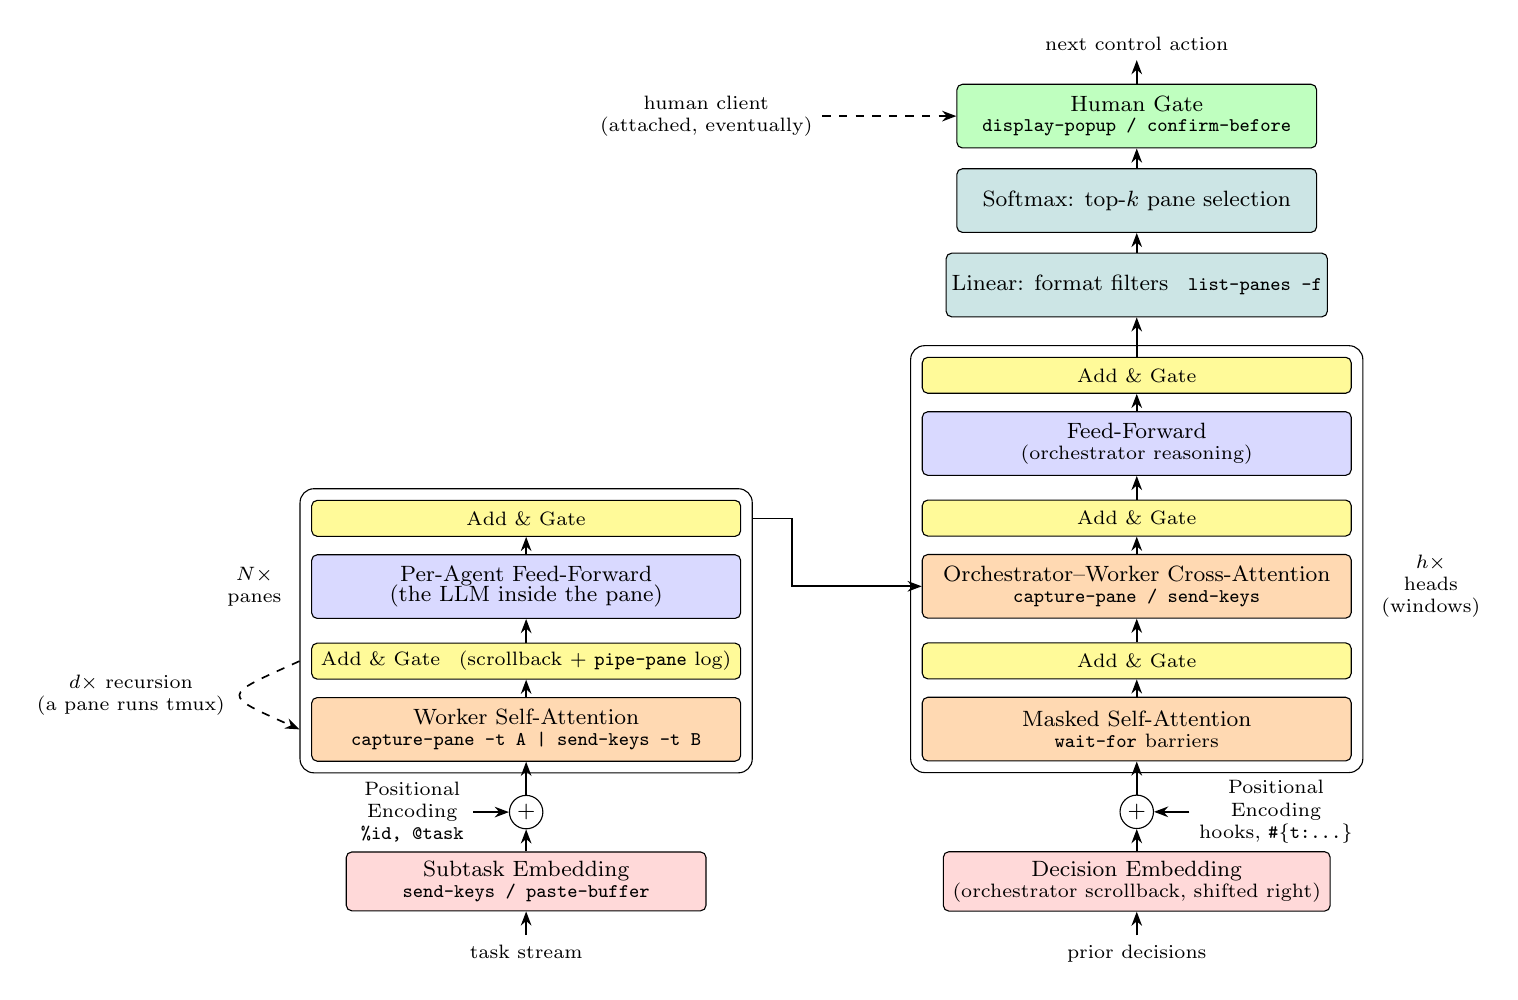
\begin{tikzpicture}[font=\footnotesize,
  every node/.style={align=center},
  attn/.style={draw, rounded corners=2pt, fill=orange!30, minimum width=15.5em, minimum height=2.3em, inner sep=2pt},
  ffn/.style={attn, fill=blue!15},
  addg/.style={draw, rounded corners=2pt, fill=yellow!40, minimum width=15.5em, minimum height=1.3em, font=\scriptsize, inner sep=2pt},
  emb/.style={draw, rounded corners=2pt, fill=red!15, minimum width=13em, minimum height=2.1em},
  gate/.style={attn, fill=green!25},
  soft/.style={attn, fill=teal!20},
  plus/.style={draw, circle, inner sep=1.2pt},
  arr/.style={-{Stealth[length=1.8mm]}, semithick},
  darr/.style={arr, dashed}]

% ---------------- encoder (worker) column ----------------
\node[emb] (eemb) at (0,0) {Subtask Embedding\\[-2pt]{\ttfamily\scriptsize send-keys / paste-buffer}};
\node[plus, above=0.28cm of eemb] (eplus) {$+$};
\node[attn, above=0.42cm of eplus] (eatt) {Worker Self-Attention\\[-2pt]{\ttfamily\scriptsize capture-pane -t A | send-keys -t B}};
\node[addg, above=0.22cm of eatt] (eadd1) {Add \& Gate \enspace(scrollback $+$ {\ttfamily pipe-pane} log)};
\node[ffn, above=0.3cm of eadd1] (effn) {Per-Agent Feed-Forward\\[-2pt](the LLM inside the pane)};
\node[addg, above=0.22cm of effn] (eadd2) {Add \& Gate};
\node[draw, rounded corners=5pt, fit=(eatt)(eadd2), inner sep=0.4em] (encbox) {};
\node[font=\scriptsize, anchor=east, xshift=-3pt] at (encbox.west |- effn) {$N\times$\\panes};

% ---------------- decoder (orchestrator) column ----------------
\node[emb, right=3.0cm of eemb] (demb) {Decision Embedding\\[-2pt]{\scriptsize(orchestrator scrollback, shifted right)}};
\node[plus, above=0.28cm of demb] (dplus) {$+$};
\node[attn, above=0.42cm of dplus] (datt1) {Masked Self-Attention\\[-2pt]{\ttfamily\scriptsize wait-for} {\scriptsize barriers}};
\node[addg, above=0.22cm of datt1] (dadd1) {Add \& Gate};
\node[attn, above=0.3cm of dadd1] (datt2) {Orchestrator--Worker Cross-Attention\\[-2pt]{\ttfamily\scriptsize capture-pane / send-keys}};
\node[addg, above=0.22cm of datt2] (dadd2) {Add \& Gate};
\node[ffn, above=0.3cm of dadd2] (dffn) {Feed-Forward\\[-2pt]{\scriptsize(orchestrator reasoning)}};
\node[addg, above=0.22cm of dffn] (dadd3) {Add \& Gate};
\node[draw, rounded corners=5pt, fit=(datt1)(dadd3), inner sep=0.4em] (decbox) {};
\node[font=\scriptsize, anchor=west, xshift=3pt] at (decbox.east |- datt2) {$h\times$\\heads\\(windows)};

% ---------------- output head ----------------
\node[soft, above=0.5cm of dadd3, minimum width=13em] (lin) {Linear: format filters \enspace{\ttfamily\scriptsize list-panes -f}};
\node[soft, above=0.25cm of lin, minimum width=13em] (smax) {Softmax: top-$k$ pane selection};
\node[gate, above=0.25cm of smax, minimum width=13em] (hgate) {Human Gate\\[-2pt]{\ttfamily\scriptsize display-popup / confirm-before}};
\node[font=\scriptsize, above=0.3cm of hgate] (out) {next control action};

% ---------------- arrows ----------------
\node[font=\scriptsize, below=0.3cm of eemb] (etask) {task stream};
\node[font=\scriptsize, below=0.3cm of demb] (dtask) {prior decisions};
\draw[arr] (etask) -- (eemb);
\draw[arr] (eemb) -- (eplus);
\draw[arr] (eplus) -- (eatt);
\draw[arr] (eatt) -- (eadd1);
\draw[arr] (eadd1) -- (effn);
\draw[arr] (effn) -- (eadd2);
\draw[arr] (dtask) -- (demb);
\draw[arr] (demb) -- (dplus);
\draw[arr] (dplus) -- (datt1);
\draw[arr] (datt1) -- (dadd1);
\draw[arr] (dadd1) -- (datt2);
\draw[arr] (datt2) -- (dadd2);
\draw[arr] (dadd2) -- (dffn);
\draw[arr] (dffn) -- (dadd3);
\draw[arr] (dadd3) -- (lin);
\draw[arr] (lin) -- (smax);
\draw[arr] (smax) -- (hgate);
\draw[arr] (hgate) -- (out);

% cross-attention feed: encoder output -> decoder cross-attention
\draw[arr] (encbox.east |- eadd2) -- ++(0.5,0) |- (datt2.west);

% positional encodings
\node[font=\scriptsize, left=0.45cm of eplus] (epe) {Positional\\Encoding\\{\scriptsize\ttfamily \%id, @task}};
\draw[arr] (epe) -- (eplus);
\node[font=\scriptsize, right=0.45cm of dplus] (dpe) {Positional\\Encoding\\{\scriptsize hooks, \ttfamily \#\{t:\ldots\}}};
\draw[arr] (dpe) -- (dplus);

% recursion loop on the encoder stack
\draw[darr] (encbox.west |- eadd1) .. controls +(-1.0,-0.45) and +(-1.0,0.45) .. (encbox.west |- eatt)
  node[midway, left, font=\scriptsize, align=center, xshift=-2pt] {$d\times$ recursion\\{\scriptsize(a pane runs tmux)}};

% the human attaches at the gate
\draw[darr] ([xshift=-1.7cm]hgate.west) -- (hgate.west)
  node[at start, anchor=east, font=\scriptsize, align=center] {human client\\{\scriptsize(attached, eventually)}};
\end{tikzpicture}}
\caption{The Tmux Orchestration Architecture, drawn in the family style. Worker panes
(left, the encoder stack) and the orchestrator (right, the decoder) exchange
information through \code{capture-pane}/\code{send-keys} cross-attention;
\code{wait-for} masks the orchestrator's self-attention; the human gate sits where
the softmax used to be.}
\label{fig:arch}
\end{figure}

\subsection{Session, Window, and Pane Stacks}\label{sec:stacks}

The encoder and decoder are composed of a stack of identical structural layers,
provided by tmux's three-level hierarchy:

\begin{itemize}
\item \textbf{Server} --- one per socket (\code{-L name} / \code{-S /path/socket}), a
namespace holding all sessions. Distinct sockets give separate servers whose
sessions, channels, and options cannot collide --- \emph{namespace separation},
which must not be mistaken for a sandbox. Every server runs as the same user on the
same filesystem with the same credentials, and any process of that user may connect
to any socket it can name. Confining an untrusted agent takes an OS boundary (a
separate user, container, or VM) and credential scoping; tmux contributes tidiness,
not security.
\item \textbf{Session} --- a durable collection of windows, detachable from any client.
One session per project or major objective.
\item \textbf{Window} --- a full-screen layer within a session, tiled into panes. One
window per orchestration \emph{head} (\S\ref{sec:mha}) or per phase.
\item \textbf{Pane} --- a single pseudo-terminal running exactly one agent process. The
pane is the atomic unit: the residence of one Claude Code or Codex session.
\end{itemize}

Each worker pane is wrapped by two connections analogous to the residual connection
and layer normalization around each Transformer sub-layer. A \emph{residual path}:
the pane's scrollback and, optionally, an append-only log via
\code{pipe-pane -o -t <pane> 'cat >> log'}, which streams output to a file for the
pane's lifetime, so context flows \emph{around} each interaction:
$\mathrm{LayerOutput} = \mathrm{Agent}(x) + x$, where $x$ is the durable prior
context. And a \emph{normalization gate}: a checkpoint at which the orchestrator or
human inspects and, if necessary, constrains the pane's output before it propagates
--- the human-in-the-loop gate of \S\ref{sec:reg}, bounding an agent's divergence
before it affects shared state. The output of each sub-layer is thus
$\mathrm{Gate}\!\left(x + \mathrm{Agent}(x)\right)$, with $\mathrm{Agent}$
implemented by the LLM inside the pane and $\mathrm{Gate}$ by the review policy.

\subsection{Attention}

An orchestration attention function maps a \emph{query} (the orchestrator's current
subgoal) and a set of \emph{key--value} pairs (the addressable worker panes and their
captured contents) to an output (the next control action). Let the swarm be a set of
panes $P = \{p_1,\dots,p_n\}$. Each pane exposes, via tmux \emph{format variables}, a
\textbf{key} $k_i$ (its addressable, queryable metadata) and a \textbf{value} $v_i$
(its current content):

\begin{lstlisting}
k_i = ( #{pane_id}, #{@role}, #{@task_id}, #{@state},
        #{pane_current_command}, #{pane_title},
        #{pane_dead}, #{window_silence_flag} )
v_i = capture-pane -p -t "#{pane_id}"
\end{lstlisting}

The address in every key is \code{pane\_id} --- the immutable \code{\%N} the server
assigns at creation --- never a window/pane \emph{index}, which is a presentation
coordinate that renumbers under topology changes (\S\ref{sec:pe}). The keys are
cheaply enumerable for the whole swarm in a single call:

\begin{lstlisting}
tmux list-panes -a -F '#{pane_id} role=#{@role} state=#{@state} \
  cmd=#{pane_current_command} dead=#{pane_dead}'
\end{lstlisting}

\begin{figure}[t]
\centering
\begin{minipage}[b]{0.44\textwidth}
\centering
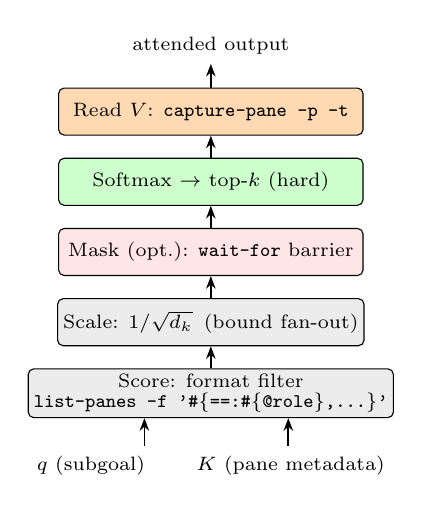
\begin{tikzpicture}[font=\scriptsize, every node/.style={align=center},
  box/.style={draw, rounded corners=2pt, minimum width=11em, minimum height=1.7em, inner sep=2pt},
  arr/.style={-{Stealth[length=1.6mm]}, semithick}]
\node[box, fill=gray!15] (score) {Score: format filter\\[-1pt]{\ttfamily list-panes -f '\#\{==:\#\{@role\},...\}'}};
\node[box, fill=gray!15, above=0.28cm of score] (scale) {Scale: $1/\sqrt{d_k}$ \,(bound fan-out)};
\node[box, fill=pink!40, above=0.28cm of scale] (mask) {Mask (opt.): {\ttfamily wait-for} barrier};
\node[box, fill=green!20, above=0.28cm of mask] (smax) {Softmax $\rightarrow$ top-$k$ (hard)};
\node[box, fill=orange!30, above=0.28cm of smax] (cap) {Read $V$: {\ttfamily capture-pane -p -t}};
\node[below=0.35cm of score] (qk) {$q$ (subgoal) \qquad $K$ (pane metadata)};
\draw[arr] ([xshift=-2.4em]qk.north) -- ([xshift=-2.4em]score.south);
\draw[arr] ([xshift=2.8em]qk.north) -- ([xshift=2.8em]score.south);
\draw[arr] (score) -- (scale);
\draw[arr] (scale) -- (mask);
\draw[arr] (mask) -- (smax);
\draw[arr] (smax) -- (cap);
\node[above=0.3cm of cap] (o) {attended output};
\draw[arr] (cap) -- (o);
\end{tikzpicture}
\end{minipage}\hfill
\begin{minipage}[b]{0.52\textwidth}
\centering
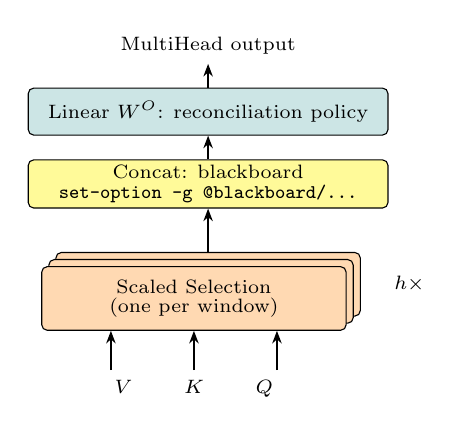
\begin{tikzpicture}[font=\scriptsize, every node/.style={align=center},
  box/.style={draw, rounded corners=2pt, minimum width=11em, minimum height=1.7em, inner sep=2pt},
  arr/.style={-{Stealth[length=1.6mm]}, semithick}]
\node[box, fill=orange!30, minimum height=2.3em] (h2) at (0.18,0.18) {};
\node[box, fill=orange!30, minimum height=2.3em] (h1) at (0.09,0.09) {};
\node[box, fill=orange!30, minimum height=2.3em] (h0) at (0,0) {Scaled Selection\\[-1pt](one per window)};
\node[right=0.3cm of h2, font=\scriptsize] (hh) {$h\times$};
\node[box, fill=yellow!40, above=0.55cm of h2, minimum width=13em] (cat) {Concat: blackboard\\[-1pt]{\ttfamily set-option -g @blackboard/...}};
\node[box, fill=teal!20, above=0.3cm of cat, minimum width=13em] (wo) {Linear $W^{O}$: reconciliation policy};
\node[below=0.5cm of h0] (vkq) {$V$ \qquad $K$ \qquad $Q$};
\draw[arr] ([xshift=-3em]vkq.north) -- ([xshift=-3em]h0.south);
\draw[arr] (vkq.north) -- (h0.south);
\draw[arr] ([xshift=3em]vkq.north) -- ([xshift=3em]h0.south);
\draw[arr] (h2.north) -- (cat);
\draw[arr] (cat) -- (wo);
\node[above=0.3cm of wo] (mo) {MultiHead output};
\draw[arr] (wo) -- (mo);
\end{tikzpicture}
\end{minipage}
\caption{(left) Scaled Selection. (right) Multi-Head Orchestration: $h$ selection
channels run in parallel windows and are combined through a shared blackboard.}
\label{fig:attn}
\end{figure}

\subsubsection{Scaled Dot-Product Attention (Scaled Selection)}\label{sec:sdpa}

We call our particular attention ``Scaled Selection.'' The input consists of a query
$q$ (the current subgoal), keys $k_i$ of dimension $d_k$ (pane metadata), and values
$v_i$ (pane contents). We compute a relevance score between the query and each pane's
key, apply a softmax to obtain weights, and read the weighted values
(Figure~\ref{fig:attn}, left):\footnote{The vector space in which terminal
scrollback admits convex combination is left as future work; in deployment the
softmax temperature is taken to zero and the sum collapses to hard selection.}
\begin{equation}
\mathrm{OrchAttention}(q,K,V) =
  \sum_{i} \mathrm{softmax}_i\!\left(\frac{\mathrm{score}(q,k_i)}{\sqrt{d_k}}\right)
  \cdot \mathrm{Capture}(p_i).
\end{equation}

In practice $\mathrm{score}(q,k_i)$ is realized as a \emph{format filter} --- a
predicate over the pane's key fields that the orchestrator evaluates with
\code{list-panes -f} / \code{if-shell -F}. For example, ``attend to reviewer workers
currently blocked at a shell prompt'':

\begin{lstlisting}
tmux list-panes -a \
  -f '#{&&:#{==:#{@role},reviewer},#{==:#{@state},idle}}' \
  -F '#{pane_id}'
\end{lstlisting}

The scaling factor $1/\sqrt{d_k}$ is where the analogy is at its most decorative,
and we say so plainly: multiplying every score by the same positive constant changes
no ranking, so it cannot change what any hard top-$k$ selects. What the factor
guards in the original --- selection staying sharp as dimensionality grows --- is
real here, but it is enforced by choosing $k$, the per-step fan-out, small and
fixed. In deployment the ``softmax'' is a Boolean format predicate over pane keys
followed by a capped number of reads: filter, then bound. Where genuine ranking is
wanted (most-recently-quiet first, longest-blocked first), the orchestrator computes
a numeric score per pane and sorts --- tmux supplies the fields (\code{\#\{t:...\}}
timestamps, user options), not the ordering. Reading a value is
\code{capture-pane}; writing to the selected panes is \code{send-keys}, with a
paste-buffer path for large or special-character payloads --- one uniquely named
buffer per task, deleted on paste, so concurrent dispatches cannot race on a shared
buffer name:

\begin{lstlisting}
tmux capture-pane -p -t "$target" -S -200              # READ  (the "V")
tmux send-keys    -t "$target" "run the tests" Enter   # WRITE (route subgoal)
tmux load-buffer  -b "task-$id" ./subtask-prompt.txt   # large payload, no escaping
tmux paste-buffer -d -b "task-$id" -t "$target"        # unique buffer, freed on paste
\end{lstlisting}

Two practical notes. First, \code{send-keys} interprets key names --- \code{Enter},
\code{C-c} --- so literal payloads should be sent with \code{-l}, lest a string
containing ``Enter'' be helpfully pressed on the worker's behalf. Second, keys land
in whatever the pane is doing \emph{right now}; dispatch is therefore gated on the
worker being at rest (\S\ref{sec:pe}), since injecting a subtask into an agent
mid-generation adds noise without gradient.

\subsubsection{Multi-Head Orchestration}\label{sec:mha}

Rather than run a single orchestration channel over the full swarm, we found it
beneficial to run $h$ channels in parallel --- one per tmux \textbf{window} --- each
with its own selection projection (its own \code{@role} filter, subset of the swarm,
and subgoal). Each head $i$ attends independently (Figure~\ref{fig:attn}, right),
\begin{equation}
\mathrm{head}_i = \mathrm{OrchAttention}\!\left(qW_i^{Q},\, KW_i^{K},\, VW_i^{V}\right),
\end{equation}
where the projections $W_i$ are, concretely, the per-window scoping of which panes and
key fields that head considers relevant. Multi-head orchestration lets the
architecture jointly attend to different parts of the project at different phases:
head 1 supervises implementation panes, head 2 a test/CI pane, head 3 documentation,
head 4 a long-running build. We are careful about where the concurrency lives: the
\emph{workers} under each head run concurrently as independent OS processes, but a
single orchestrator walking the windows remains one decision process, time-slicing
its own attention --- a window is an organizational scope, not a thread.
Decision-level parallelism requires one orchestrator process per head, which is
exactly the recursion of \S\ref{sec:why}: a head that matters enough is given its
own sub-orchestrator pane. The heads are
combined by concatenation into a shared \textbf{blackboard} --- persistent key/value
state in tmux user-options, readable and writable by any head:

\begin{lstlisting}
tmux set-option  -g @blackboard/build_status "green"   # write  (Concat)
tmux show-option -gv @blackboard/build_status          # read
\end{lstlisting}

$\mathrm{MultiHead} = \mathrm{Concat}(\mathrm{head}_1,\dots,\mathrm{head}_h)\,W^{O}$,
where $W^{O}$ is the reconciliation policy that resolves conflicting writes
(last-writer-wins, or an orchestrator-mediated merge).

\subsubsection{Applications of Attention in Our Model}

The architecture uses orchestration attention in three ways. \textbf{(1)
Orchestrator$\to$worker cross-attention:} the decoder queries over all worker panes,
reading their captured state and writing their next instruction --- the analog of
encoder--decoder attention, via addressed reads and writes on stable pane IDs.
\textbf{(2) Worker self-attention:} workers attend to one another \emph{without}
routing through the orchestrator when a direct pipe is authorized,
\code{capture-pane -p -t A | ... | send-keys -t B}. \textbf{(3) Masked orchestrator
self-attention:} the orchestrator attends to its own prior decisions (scrollback,
blackboard) to remain autoregressive, but is \emph{masked} from depending on subtasks
that have not yet completed. The mask is enforced with \code{wait-for}: a barrier that
blocks the orchestrator from consuming a result until the producing worker signals
completion (\S\ref{sec:ffn}), preserving the auto-regressive property.

\subsection{Position-wise Feed-Forward Networks (Per-Agent Reasoning and Barriers)}\label{sec:ffn}

In addition to attention sub-layers, each pane contains a fully-connected
feed-forward network applied to that position independently: the LLM inference
performed \emph{inside} the agent. This is the actual ``thinking'' --- identical in
form at every pane but with different, per-pane parameters (the agent's own context
window and system prompt). Synchronization between the attention layer and these
per-agent computations is provided by \code{wait-for}, tmux's built-in barrier/signal
channel:

\begin{lstlisting}
tmux wait-for -S subtask-42   # worker: signal completion (last line of its task)
tmux wait-for    subtask-42   # orchestrator/dependent: block until signalled
\end{lstlisting}

\code{wait-for -L} / \code{-U} additionally provide a lock/unlock primitive for mutual
exclusion over the shared working tree, preventing two workers from writing the same
files concurrently.

Two properties deserve emphasis. First, a signal on a channel with no waiter is not
lost: the server latches one wake, and the next waiter consumes it. But it is a
\emph{one-bit latch}, not a counting queue --- early signals coalesce, and a reused
channel can hand a stale wake to the wrong consumer. The discipline that follows is
one globally unique channel per task attempt
(\code{done:\$swarm:\$task:\$attempt}), never reused. Second, channels are
server-global, so recursive sub-swarms take their own sockets
(\S\ref{sec:stacks}) and collisions become impossible by construction.
\code{wait-for -L}/\code{-U}, finally, is an \emph{advisory} mutex among
cooperating scripts: nothing compels a worker to take it, and a crashed holder
releases nothing, so a real lock carries an owner record and recovery logic beside
it.

\subsection{Embeddings and Readout}

Before a subtask enters the swarm it is \emph{embedded} into the substrate: a natural
language objective is tokenized into a shell-injectable instruction and a target
address (which pane, which role). Symmetrically, the \emph{readout} projects a pane's
raw terminal output back into a decision-usable representation via \code{capture-pane}
(with \code{-e} to retain escape sequences or \code{-J} to rejoin wrapped lines). As
in the Transformer, we share the same learned mapping between the input embedding (how
we phrase instructions to agents) and the pre-readout transformation (how we parse
their replies): the orchestrator's prompt conventions and its output parser are two
directions of one shared protocol, which for control-mode clients is the
\code{\%}-prefixed structured stream itself \cite{tmuxcontrol}.

A caveat keeps this section honest. \code{capture-pane} returns the rendered grid
and retained history --- a picture of a terminal, not a message stream --- and
\code{pipe-pane} admits one pipe per pane, streaming only while attached. For an
operator's console this is exactly right; as the sole data plane of an autonomous
protocol it lacks framing, acknowledgement, and schema. Deployment therefore moves
payloads over a thin per-worker file protocol with atomic renames
(\S\ref{sec:batching}) and reserves the terminal for what it is: an attention
surface, not a message bus.

\subsection{Positional Encoding}\label{sec:pe}

The swarm, as described, is a \emph{set} of panes --- orchestration attention is
permutation-invariant and by itself carries no notion of which agent came first or
which subtask depends on which. Since dependency order matters, we must inject
information about the position of each agent in the topology and in time.

Tmux supplies identity and order natively, provided one uses the right coordinates.
Each pane has a \textbf{unique ID} (\code{\#\{pane\_id\}}, the \code{\%N} the server
assigns at creation), immutable for the pane's lifetime; sessions and windows carry
\code{\$N} and \code{@N} likewise. Window and pane \emph{indexes}, by contrast, are
presentation coordinates: they renumber under \code{break-pane}, \code{join-pane},
\code{swap-pane}, and \code{move-window} --- the very operations
\S\ref{sec:deploy} uses to reshape the swarm mid-run. Scripts therefore address
panes by ID and keep semantic position in explicit per-pane user options
(\code{@role}, \code{@task\_id}, \code{@state}); indexes are for the human's
fingers. We combine identity with a \textbf{temporal coordinate} from event hooks
and the \code{\#\{t:...\}} time formats, so each agent carries a position signal
analogous to the sinusoidal encoding, letting the orchestrator reason about
dependency order without a recurrent scan:
\[
\mathrm{PE}(\mathrm{pane}) =
  \big(\, \mathit{pane\_id},\;\; \mathit{@task\_id},\;\;
          \mathit{timestamp\ of\ last\ state\ change} \,\big).
\]
The temporal component is maintained \emph{event-drivenly} by hooks rather than by
polling:

\begin{lstlisting}
# Stamp when a pane goes quiet (a watchdog event, not a completion signal)
tmux set-hook -g alert-silence \
  'set-option -p @last_silent "#{t:window_activity}" ; run-shell "notify-orch #{pane_id}"'
# React to a worker crashing (a "position" removed from the sequence)
tmux set-hook -g pane-died \
  'run-shell "orch handle-death #{pane_id} status=#{pane_dead_status}"'
\end{lstlisting}

Available hook events include \code{pane-died}, \code{alert-activity},
\code{alert-silence}, \code{alert-bell}, \code{session-created},
\code{client-attached}, and \code{client-detached} \cite{tmuxhooks}. Note that
\code{pane-died} fires only when \code{remain-on-exit} is \code{on}, leaving the
corpse addressable for a \code{capture-pane} post-mortem before \code{respawn-pane};
with the default \code{off} the pane closes and the weaker \code{pane-exited} fires
--- the evidence leaves with it. Activity/silence monitoring is enabled with
\code{monitor-activity on} and \code{monitor-silence <seconds>} --- these are
\emph{window} options, and \code{alert-silence} fires per window, so a per-worker
silence watchdog wants one window per worker, which the multi-head layout already
provides. And it is a \emph{watchdog}, never a completion protocol: silence cannot
distinguish a finished worker from one mid-inference, blocked on the network,
deadlocked, or waiting for confirmation --- and \code{pane\_current\_command} is
only a corroborating hint, since a TUI agent stays in the foreground whether
generating or idle. Completion is therefore explicit: the worker's last act is to
set \code{@state done} and signal its unique per-attempt channel
(\S\ref{sec:ffn}); silence merely tells the orchestrator where to look when nothing
has been said for too long. This gives the swarm a \emph{positional} sense of ``who
just spoke and who just went quiet,'' computed once and event-drivenly, rather than
re-derived by a sequential human sweep.

% ==================================================================
\section{Why Tmux}\label{sec:why}

In this section we compare the tmux orchestration substrate to alternatives ---
recurrent human management and centralized-process orchestration. An earlier draft
compressed the comparison into a single ``path length''; an adversarial reviewer
correctly observed that $A \to$ relay $\to B$ is a constant number of hops however
slow the relay, and that a substrate scan such as \code{list-panes -f} is linear in
the panes inspected however few round trips it takes. We therefore separate the
metrics: \emph{human interventions} required in the inner loop; \emph{semantic
re-emissions} per data hop, the number of times a payload must cross a deciding
process --- a mind or a model --- to move between two agents; \emph{transport cost}
to reach an agent whose address is already known; and \emph{discovery cost} to find
out which agent that is.

\begin{table}[t]
\centering
\caption{Separated coordination metrics. ``Semantic re-emissions'' counts the times
a payload crosses a deciding process (a mind or a model) to move between two
agents; transport assumes the target's pane ID is already known; discovery is a
single \code{list-panes} round trip that enumerates all $n$ panes server-side.}
\label{tab:why}
\vspace{0.4em}
\resizebox{\textwidth}{!}{%
\begin{tabular}{@{}lcccc@{}}
\toprule
\textbf{Substrate} & \textbf{Human ops, inner loop} & \textbf{Sem.\ re-emissions / hop} & \textbf{Transport (known agent)} & \textbf{Discovery}\\
\midrule
Recurrent human management & every hop & 1 (the operator) & serial re-type & $O(n)$ visual scan \\
Central-process orchestrator & none & 1 (the process) & $O(1)$ IPC & process-dependent \\
\textbf{Tmux orchestration (this work)} & \textbf{gate only} & \textbf{0} on authorized pipes & $O(1)$ addressed, \code{-t \%id} & $O(n)$ scan, 1 round trip \\
\bottomrule
\end{tabular}}
\end{table}

The honest reading of Table~\ref{tab:why} is that tmux buys the two middle columns.
A data hop between workers whose IDs are known
(\code{capture-pane -t \%4 | ... | send-keys -t \%7}) crosses no deciding process
at all, where recurrent management pays the operator's working memory on every hop
and a central-process design pays a parse--decide--re-emit cycle. What tmux does
\emph{not} buy is any reduction in semantic work: it selects no recipients,
interprets no dependencies, reconciles no conflicts, and trusts no output ---
every decision still happens in the orchestrator, whose reasoning costs are
identical across substrates and appear in no column. Tmux replaces
terminal-switching and process-management labor, not judgment.

An adversarial reader will object that the tmux server is itself a single central
process. It is --- and that is the point of the middle column. The server moves
bytes between pseudo-terminals without parsing them, holds no conversation state,
and re-emits nothing through a context window, so a hop through it counts zero
semantic re-emissions. The charge against the central-process design is not that it
is central but that it is \emph{semantically} central: every payload crosses its
parse--decide--re-emit cycle whether or not that payload needed a decision.

Two further benefits motivated the choice of tmux. \textbf{Durability/detachability:}
because the server outlives its clients, the human can detach entirely and the swarm
keeps running; work is not lost on disconnect. This is what lets the human be in the
loop \emph{eventually} (\S\ref{sec:reg}) rather than \emph{always}. \textbf{Recursion:}
a pane may run a tmux client that owns its own server or session, so an orchestrator
can spawn \emph{sub-orchestrators}, each managing a sub-swarm; the addressing composes
via nested prefixes (\code{C-b C-b ...}) and per-socket namespaces. Depth-$d$ recursion
yields a coordination \emph{tree}; the human attaches only at the root and can literally
\code{choose-tree} to watch the whole hierarchy.

% ==================================================================
\section{Deployment}\label{sec:deploy}

This section describes how a swarm is decomposed, batched, scheduled, and regularized
in operation --- the ``training regime'' of the architecture.

\subsection{Task Decomposition and Batching}\label{sec:batching}

Each engineering objective is decomposed by the orchestrator into subtasks batched by
\emph{independence}: subtasks with no shared file dependency are dispatched to distinct
worker panes in the same step and proceed in parallel; dependent subtasks are
serialized behind \code{wait-for} barriers (\S\ref{sec:ffn}) and \code{wait-for -L}
locks over shared paths. Batches are sized to keep fan-out $k$ bounded
(\S\ref{sec:sdpa}) so neither the orchestrator's control bandwidth nor the human's
review bandwidth saturates.

Two further disciplines carry the batching in practice. Each worker owns a separate
Git \emph{worktree} --- a shared index turns independent subtasks into merge
conflicts you scheduled for yourself --- and payloads travel through a thin
per-worker \emph{shim}: task and result envelopes as files delivered by atomic
rename, with the pane's terminal carrying the agent's face rather than the freight.
Tmux wakes, supervises, and displays; the files remember.

\subsection{Hardware and Schedule}

A swarm runs on a single host (or a \code{tmux -S} socket shared over SSH), one pane
per worker process. The orchestrator loop alternates between an \emph{event-driven}
phase --- blocking on hooks and \code{wait-for} signals, consuming near-zero CPU while
workers think --- and a \emph{dispatch} phase triggered when a pane goes silent, dies,
or signals completion. Control mode (\code{-CC}) is used when the orchestrator is
itself an agent: it reads the \code{\%}-prefixed notification stream (\code{\%output},
\code{\%window-pane-changed}, \code{\%exit}, \dots) directly rather than
screen-scraping \cite{tmuxcontrol}. A production control-mode client is real
engineering, not a line-oriented loop: it must correlate
\code{\%begin}/\code{\%end}/\code{\%error} responses with the commands that caused
them, tolerate escaped and non-UTF-8 output, honor the protocol's flow control so a
slow reader does not fall behind, and resynchronize with \code{capture-pane} after
a disconnect. We use the notification stream for wakes and supervision, keep
payloads on the file protocol of \S\ref{sec:batching}, and declare a fully general
control-mode parser future work.

\subsection{Optimizer (the Control Loop)}

The orchestration policy is the ``optimizer'' driving the swarm toward the objective.
We use an event-driven loop with bounded polling as a fallback:

\begin{lstlisting}
loop:
  wait on { hooks(pane-died, alert-silence), wait-for signals }   # event-driven
  on signal from pane p:
     v <- capture-pane(p)                     # attend (read)
     decision <- orchestrator.step(q, v)      # per-agent FFN of the decoder
     apply(decision):                         # attend (write)
        send-keys / paste-buffer to selected panes   # continue work
        respawn-pane p                                # restart a crashed worker
        break-pane / join-pane / swap-pane            # reshape topology
        set-option @blackboard/...                    # update shared state
     if decision.needs_human: escalate_to_gate()      # see 5.4
\end{lstlisting}

We adopt a schedule analogous to warmup-then-decay: early in an objective the
orchestrator polls more aggressively and escalates to the human more readily
(\emph{warmup} --- establishing shared context and trust); as the objective stabilizes
it relies more on event-driven hooks and widens the human-gate interval
(\emph{decay}). \code{respawn-pane}/\code{respawn-window} provide restart-on-failure,
and \code{break-pane}/\code{join-pane} let the optimizer restructure the swarm topology
mid-run.

\subsection{Regularization (Human-in-the-Loop Gate)}\label{sec:reg}

We employ several regularizers to prevent the swarm from overfitting to a locally
plausible but globally wrong plan. \textbf{Human-gate:} the single most important
regularizer, and the easiest to fake. A popup is an interface, not an enforcement
mechanism --- with no client attached there is nowhere to draw it, and a worker
holding push credentials needs nobody's permission. The gate is therefore a
\emph{capability boundary}. Workers run without credentials for protected
operations (a push, a deploy, a destructive command); a request for one is
persisted to disk and the swarm moves on; the human reviews pending requests on
attach, with \code{display-popup} and \code{choose-tree} as how the queue looks,
not why it holds; and a broker that alone holds the credentials validates and
executes the exact approved command. Direct worker-to-worker pipes
(\S 3.2.3) carry data, never authority. The human is thus in the loop
\emph{eventually and where it matters}, not in every inner iteration --- the analog
of applying regularization at the layer boundaries rather than to every activation.
\textbf{Silence dropout:} panes silent beyond a threshold are treated as dropped for
the current step (\code{monitor-silence}), forcing the orchestrator not to rely on any
single worker always being available. \textbf{Checkpoint/residual:} \code{pipe-pane}
logs and periodic git commits provide the residual path that lets the swarm recover
context after a crash or a bad step.

% ==================================================================
\section{Results}

We report qualitative and illustrative operational results; a rigorous benchmark of
swarm throughput across task suites is left to future work, and the figures below are
illustrative of the regime rather than a controlled measurement. The benchmark that
would settle it is well-defined --- dispatch and result latency, false-completion
rate under the silence watchdog, recovery time after worker and orchestrator
crashes, and merge-conflict rate of shared trees versus per-worker worktrees ---
and this section's claims should be read as bounded by it.

\paragraph{Orchestration throughput.} Replacing the human relay with addressed pane
operations removes the human from the inner loop, so wall-clock throughput can scale
with \emph{available parallel workers} rather than \emph{human cycle time} --- for
genuinely independent tasks, and only until something else binds: review bandwidth
at the gate (\S\ref{sec:reg}), CPU, API rate limits, repository contention, or the
test infrastructure. Parallelism is a ceiling, not a guarantee. Within it, a single
operator supervises a swarm whose aggregate rate is set by $k$ concurrent agents
rather than by one, minus everything the previous sentence lists.

\paragraph{Architecture variations.} Table~\ref{tab:var} varies the number of heads
$h$, per-step fan-out $k$, recursion depth $d$, and the human gate. Removing the
scaling discipline on fan-out (row B) degrades supervisory quality --- the operator
cannot review 12 parallel decision streams --- and removing the human gate entirely
(row D) maximizes raw speed while forfeiting the regularization that keeps the swarm
aligned with intent. Deep recursion (row C) is the most capable configuration but
concentrates oversight at the root, recommended only once trust in the lower levels is
established.

\begin{table}[t]
\centering
\caption{Variations on the Tmux Orchestration Architecture. $h$ = orchestration heads
(windows), $k$ = per-step fan-out, $d$ = recursion depth.}
\label{tab:var}
\vspace{0.4em}
\begin{tabular}{@{}llcccl@{}}
\toprule
 & $h$ & $k$ & $d$ & \textbf{Human gate} & \textbf{Notes}\\
\midrule
base            & 3 & 4  & 1 & on irreversible ops & balanced; recommended default \\
(A) single-head & 1 & 4  & 1 & same                & simpler; loses phase separation \\
(B) wide fan-out& 3 & 12 & 1 & same                & saturates review bandwidth; thrash \\
(C) deep recursion & 3 & 4 & 3 & root only         & powerful; hardest to supervise \\
(D) no gate     & 3 & 4  & 1 & \textbf{off}        & fastest and least safe; not advised \\
\bottomrule
\end{tabular}
\end{table}

\paragraph{Generalization to heterogeneous agents.} Because the substrate addresses
\emph{panes}, not model APIs, the architecture generalizes across agent types without
modification: a pane may hold Claude Code, a Codex session, a plain REPL, or a build
process, all attended to through the same \code{send-keys}/\code{capture-pane}
interface. The orchestrator need not know what runs inside a pane, only its address and
its \code{@role} --- the substrate is model-agnostic.

% ==================================================================
\section{Conclusion}

We presented the Tmux Orchestration Architecture, a model for supervising coding-agent
swarms based entirely on the terminal multiplexer, replacing recurrent human
management with direct, addressable attention between agents. For orchestration tasks,
a single agent driving a tmux swarm connects any two workers in $O(1)$ operations,
removes the human from the inner loop, and --- by virtue of the server outliving its
clients and panes being able to run tmux themselves --- supports detachable, recursive,
semi-autonomous operation with the human retained as a supervisory gate. We plan to
apply it to swarms larger than a single host (federating over \code{tmux -S} sockets
and SSH), to learned selection policies that replace hand-written format filters, and
to tighter human-gate ergonomics. We make one claim, plainly, and scope it
honestly: for the \emph{supervision layer} --- keeping many coding agents alive,
addressable, observable, and interruptible under one human --- \textbf{tmux is all
you need}. For state, transport, and authority, tmux is precisely what you should
not use; knowing which layer you are standing in is the architecture.

\paragraph{Acknowledgements.} To every worker pane that went silent at exactly the
right moment, and to the human who stayed in the loop, eventually.

% ==================================================================
\begin{thebibliography}{9}
\small
\bibitem{bahdanau2015} D.~Bahdanau, K.~Cho, Y.~Bengio.
  \emph{Neural Machine Translation by Jointly Learning to Align and Translate.} ICLR, 2015.
\bibitem{hochreiter1997} S.~Hochreiter, J.~Schmidhuber.
  \emph{Long Short-Term Memory.} Neural Computation, 1997.
\bibitem{sutskever2014} I.~Sutskever, O.~Vinyals, Q.~V.~Le.
  \emph{Sequence to Sequence Learning with Neural Networks.} NeurIPS, 2014.
\bibitem{vaswani2017} A.~Vaswani, N.~Shazeer, N.~Parmar, J.~Uszkoreit, L.~Jones,
  A.~N.~Gomez, {\L}.~Kaiser, I.~Polosukhin.
  \emph{Attention Is All You Need.} NeurIPS, 2017.
\bibitem{yao2023} S.~Yao, J.~Zhao, D.~Yu, N.~Du, I.~Shafran, K.~Narasimhan, Y.~Cao.
  \emph{ReAct: Synergizing Reasoning and Acting in Language Models.} ICLR, 2023.
\bibitem{tmuxman} N.~Marriott et al. \emph{tmux --- terminal multiplexer, tmux(1) manual page.}
  \url{https://man7.org/linux/man-pages/man1/tmux.1.html}
\bibitem{tmuxcontrol} tmux project. \emph{Control Mode.} tmux/tmux Wiki.
  \url{https://github.com/tmux/tmux/wiki/Control-Mode}
\bibitem{tmuxhooks} tmux project. \emph{Hooks and Notifications.} tmux/tmux documentation.
\end{thebibliography}

% ==================================================================
\appendix
\section{Minimal Reproducible Swarm}

A minimal two-worker swarm --- session, per-worker windows, stable pane IDs,
watchdogs, and explicit completion --- expressed entirely in tmux. It is a
supervisor and a console, not a full orchestrator: scheduling policy, the worker
shim of \S\ref{sec:batching}, and the credential broker of \S\ref{sec:reg} live
outside it. A maintained version, with a pane registry, event log, and demo mode,
ships alongside this paper as \code{swarm/swarm.sh}.

\begin{lstlisting}
#!/usr/bin/env bash
set -euo pipefail
SOCK="swarm"; LOG="$PWD/logs"; mkdir -p "$LOG"
T() { tmux -L "$SOCK" "$@"; }

# 1. Durable, detached session; corpses stay addressable (pane-died needs it).
T new-session -d -s proj -n orch
T set-option -g remain-on-exit on
T set-option -p -t proj:orch.0 @role orchestrator

# 2. One window per worker (per-worker silence watchdog); record stable pane IDs.
for w in 0 1; do
  id=$(T new-window -dP -t proj -n "w$w" -F '#{pane_id}')
  T set-option -p -t "$id" @role worker ; T set-option -p -t "$id" @state idle
  T pipe-pane   -o -t "$id" "cat >> '$LOG/worker-$w.log'"
  T set-option  -w -t "proj:w$w" monitor-silence 20   # watchdog, NOT completion
  T send-keys -t "$id" -l 'claude' ; T send-keys -t "$id" Enter
  echo "$w $id" >> "$LOG/registry"                    # index -> immutable %id
done

# 3. Watchdog events land in an append-only log the orchestrator tails.
T set-hook -g alert-silence "run-shell \"echo silence #{pane_id} >> '$LOG/events'\""
T set-hook -g pane-died     "run-shell \"echo died #{pane_id} #{pane_dead_status} >> '$LOG/events'\""

# 4. Address by %id; completion is explicit, unique per attempt, never inferred.
dispatch() { T send-keys -t "$1" -l "$2" ; T send-keys -t "$1" Enter ; }
read_pane(){ T capture-pane -p -J -t "$1" -S -200 ; }
await()    { T wait-for  "done:$1" ; }    # one-bit latch: one channel per attempt
finish()   { T set-option -p -t "$TMUX_PANE" @state done
             T wait-for -S "done:$1" ; }  # a worker's last act, run in its pane

# 5. The human attaches at the root; detaching stops nothing. The gate of 5.4
#    is a credential broker, not a function this script could contain.
#    tmux -L swarm attach -t proj      # choose-tree (C-b s / C-b w) to watch heads
\end{lstlisting}

\end{document}
